	\subsection{Прямое произведение проективных многообразий}\label{dir_prod}

    \hypertarget{bilet_20}{}

	В этом параграфе мы построим произведение квазипроективных многообразий, как квазипроективное подмногообразие в $\PP^N$ для некоторого $N$\footnote{Тут можно дописать всякой идеологии, я это позже сделаю возможно. }

	Рассмотрим сначала $X = \PP^n, \ Y = \PP^m$. Построим вложение 
	\[
		\psi\colon \PP^n \times \PP^{(n + 1)(m + 1) - 1}
	\]
	следующим образом. Пусть $x = (u_0 : \ldots : u_n) \in \PP^n, \ y = (v_0 : \ldots : v_m)$,  тогда положим 
	\[
		\psi(x \times y) = (\ldots : w_{i j} : \ldots), \text{ где } w_{i j} = u_i v_j.
 	\]

 	Обозначим $T = \psi(\PP^n \times \PP^m)$. Во-первых, покажем, что $T$~--- замкнутое множество в $\PP^{(n + 1)(m + 1) - 1}$, для этого выпишем его уравнения: 
 	\begin{equation}
 		w_{i j} w_{k \ell} = w_{k j} w_{i \ell}, \quad i, k = 0, \ldots, n, \quad j, \ell = 0, \ldots, m. \label{Segre_embedding}
 	\end{equation}
 	Действительно, подставим: 
 	\[
 		(u_i v_j) (u_k v_\ell) = (u_k v_j) (u_i v_{\ell}),
 	\]
 	что выполнено. С другой же стороны, если $w_{i j}$ удовлетворяют уравнениям~\eqref{Segre_embedding} и, к примеру, $w_{0 0} \neq 0$, то, полагая $k = \ell = 0$, мы получаем, что  
 	\[
 		(\ldots : w_{i j} : \ldots ) = \psi(x, y),
 	\]
 	где $x = (w_{0 0}, \ldots, w_{n 0}), \ y = (w_{0 0}, \ldots, w_{0 m})$ (так мы заодно проверили, что отображение биективно). Итак, $T$~--- проективное многообразие. Построим теперь проекции: 

 	\begin{center}
 		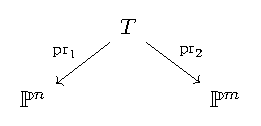
\includegraphics{lectures/5/pictures/cd_5.pdf}
 	\end{center}

 	Если $\exists i\colon u_{i j} \neq 0$:
 	\[
 		\pr_1(\ldots : w_{i j} : \ldots ) = (w_{0 j} : w_{1 j} : \ldots : w_{n j}) = (u_{0} v_j : u_{1} v_j : \ldots : u_{n} v_j) = (u_0 : \ldots : u_n).
 	\]
 	И, если $\exists j\colon u_{i j} \neq 0$:
 	\[
 		\pr_2(\ldots : w_{i j} : \ldots) = (w_{i 0} : w_{i 1} : \ldots : w_{i m}) = (u_i v_0 : u_i v_1 : \ldots u_i v_m) = (v_0 : \ldots : v_m).
 	\]

 	\begin{remark}
 		Отметим, что $\pr_1, \ \pr_2$~--- морфизмы проективных многообразий. 
 	\end{remark}

 	Тогда у нас есть композиция 
 	\[
 		\PP^m \times \PP^n \xrightarrow{\psi} T \xrightarrow{\pr_1 \times \pr_2} \PP^m \times \PP^n.
 	\]

 	Посмотрим, что произойдёт, если мы рассмотрим $T \xrightarrow{\pr_1 \times \pr_2} \PP^m \times \PP^n \xrightarrow{\psi} \PP^{(n +1)(m + 1) - 1}$:
 	\[
 		(\ldots : w_{i j} : \ldots) \mapsto (w_{0 j} : w_{1 j} : \ldots : w_{n j} : w_{i 0} : w_{i 1} : \ldots : w_{i m}) \mapsto (w_{j 0} w_{i 0} : w_{0 j} w_{i 1} : \ldots w_{0 j} w_{i m} : w_{1 j} w_{i 0} : \ldots ),
 	\]

 	И, нетрудно показать, что полученный объект снова удовлетворяет уравнениям для $T$. 

    \hypertarget{bilet_21}{}

 	\begin{definition} 
 		Пусть $X \subset \PP^n, \ Y \subset \PP^m$~--- квазипроективные многообразия, а $\psi \colon \PP^n \times \PP^m \to \PP^{(n + 1)(m + 1) - 1}$~--- определённое выше вложение\footnote{Его еще называют \emph{вложением Сегре}. }

 		Тогда определим \emph{прямое произведение} $X$ и $Y$ следующим образом: 
 		\[
 			X \times Y \eqdef \psi(X \times Y),
 		\]
 		где в правой части равенства подразумевается теоретико-множественное декартово произведение. 
 	\end{definition}

 	\begin{statement} 
 		Определение выше корректно, то есть $X \times Y$ является квазипроективным подмногообразием в $\PP^{(n + 1)(m + 1) - 1}$.
 	\end{statement}
 	\begin{proof}
 		\bf{\RNum{1}. } Пусть сначала $X \subset \PP^m$ и $Y \subset \PP^n$~--- проективные. Пусть $X$ задаётся уравнениями $F_{i}(x_0 : \ldots : x_m)$, а $Y$~--- уравнениями $G_{j}(y_0 : \ldots v_n)$. Пусть $x_0^{k_0} \ldots x_m^{k_m}$~--- какой-то моном из $F_i$, $k_0 + \ldots + k_m = N$, тогда 
 		\[
 			x_0^{k_0} \ldots x_m^{k_m} \cdot y_0^N = (x_0 y_0)^{k_0} \cdot \ldots (x_m y_0)^{k_m} = w_{00}^{k_0} \cdot \ldots \cdot w_{m 0}^{k_m}.
 		\]
 		Аналогично мы можем сделать с любым мономом. Значит, $F_i \cdot y_0^N$~---- однородный многочлен от $w_{i j}$. Также мы можем рассмотреть и $G_{j} x_i^{M}$. Так мы получаем систему из уравнений 
 		\[
 			\begin{cases}  F_i(x_0 : \ldots : x_m) y_k^N = 0 \\ \vdots \\ G_j(y_0 : \ldots : y_n) x_r^N = 0 \end{cases}, \quad 0 \le k \le n, \quad 0 \le r \le m.
 		\]
 		$N$ тут можно полагать одним и тем же, переходя к произведению. 

 		Эта система и задаёт $\psi(X \times Y)$, как проектвное подмногообразие в $\PP^{(n + 1)(m + 1) - 1}$.

 		\bf{\RNum{2}.} Теперь пусть $X, Y$~--- квазипроективные. Пусть $Y \subset Y', \ X \subset X'$, где $X', Y'$~--- проективные. Тогда $X = X' \cap U, \ Y = Y' \cap V$, где $U \subset \PP^m, \ V \subset \PP^n$~--- открытые подмножества. Тогда, так как $\psi$ инъективно (это мы видели в начала параграфа) 
 		\[
 			\psi(X \times Y) = \psi(X' \times Y') \setminus \lr*{\psi(X' \times (Y' \setminus V)) \cup \psi((X' \setminus U) \times Y') }.
 		\]
 		Заметим, что каждое из множеств в правой части замкнуто, откуда видно, что $\psi(X \times Y)$~--- октрытое модмножество $\psi(X' \times Y')$, то есть квазипроективное подмногообразие в $\PP^{(n + 1)(m + 1) - 1}$.
 	\end{proof}

 	\begin{statement} 
 		Построенное нами выше произведение является произведением в категорном смысле. 
 	\end{statement}
 	\begin{proof}
 		Мы хотим построить стрелку $\gamma\colon Z \to T$, замыкающую диаграмму и показать её единственность: 

 		\begin{center}
 			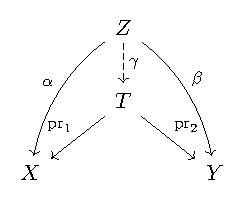
\includegraphics{lectures/5/pictures/cd_6.pdf}
 		\end{center}

 		Единственность очевидна сразу, так как $T$ также будет произведением в категории $\Set$ (откуда ясно, что на уровне множеств таких стрелок не более одной). Так вот, в качестве стрелки $\gamma$ возьмём стрелку, замыкающую диаграмму в категории $\Set$ и покажем, что она годится. Проверять, что это морфизм квазипроективных многообразий мы будем локально. 

 		Рассмотрим $z \in Z$, не умаляя общности $\alpha(z)$ и $\beta(z)$ лежат в аффинных картах и первая координата у них ненулевая. Тогда в окрестности $U \ni z$:
 		\[
 			\alpha(z') = (1 : f_1(z') : \ldots : f_m(z')), \text{ где } f_i \text{ регулярны в } U.
  		\]
  		\[
  			\beta(z') = (1 : g_1(z') : \ldots : g_n(z')), \text{ где } g_j \text{ регулярны в } U.
  		\]
  		Соотвественно, тогда 
  		\[
  			\gamma(z') = (1 : g_1(z') : \ldots : g_n(z') : f_1(z') : f_1(z') \cdot g_1(z') : \ldots : f_i(z') g_j(z') : \ldots)
  		\]
  		будем морфизмом (так как произведение регулярных функций регулярно);. 
 	\end{proof}

 	\begin{remark}
 		В дальнейшем, мы будем писать $\PP^n \times \PP^m$ вместо $\psi(\PP^n \times \PP^m)$. 
 	\end{remark}

 	Изучим теперь, как устроены подмногообразия  $X \subset \PP^m \times \PP^n$. 

 	Пусть $X$ задаётся уравненими $F_{i}(w_{0 0} : \ldots : w_{n m}) = 0$, где $F_i$~--- однородные многочлены. Тогда после подстановки $w_{i j} = x_i \cdot y_j$ мы получим систему 
 	\[
 		G_i(u_0 : \ldots u_n; v_0 : \ldots : v_m) = 0,
 	\]
 	где $G_i$ однородны как по $u_i$, так и по $v_j$, причём степени однородности обеих систем переменных. В то же время ясно, что многочлен с таким свойством однородности всегда может быть представлен, как многочлен от произведений $u_i v_j$. Однако, если уравнения однородны как по $u_i$, так и по $u_j$, то они всегда определяют в $\PP^n \times \PP^m$ алгебраическое подмногообразие, даже если степени однородности были разными. Действительно, если $G(u_0 : \ldots u_n; v_0 : \ldots v_m)$ имеет степень однородности $r$ по $u_i$ и $s$ по $v_j$ (и, например, $r > s$), то 
 	\[
 		G = 0 \leftrightarrow \begin{cases} v_1^{r - s} G = 0 \\ \vdots \\ v_m^{r - s} G = 0  \end{cases}. 
 	\]

 	Давайте также разберёмся с этим вопросом для $\PP^n \times \AA^m$. Пусть $\AA^m \hookrightarrow U_0 \subset \PP^m$, тут оно задаётся $v_0 \neq 0$. Уравнения замкнутого подмножества в $\PP^n \times \AA^m$ имеют вид 
 	\[
 		G_i(u_0 : \ldots u_n; v_0 : \ldots : v_m) = 0.
 	\]
 	Пусть степень однородности $G_i$ по $v_0, \ldots, v_m$ равна $r_i$. Поделив уравнение на $v_0^{r_i}$ и положив $y_i = v_i/v_0$ мы получим набор уравнений 
 	\[
 		g_i(u_0 : \ldots : u_n; y_1 : \ldots : y_m) = 0,
 	\]
 	где $g_i$ однородны по $u_0, \ldots, u_n$ и, вообще говоря, неоднородны по $y_1, \ldots, y_m$. Таким образом, мы доказали такую теорему: 
 	

 	\begin{theorem}\label{closed_in_product} 
 		Подмножество $X \subset \PP^n \times \PP^m$ тогда и только тогда замкнуто, когда оно задаётся системой уравнений 
 		\[
 			G_i(u_0 : \ldots u_n; v_0 : \ldots : v_m) = 0
 		\]
 		однородных по каждой системе переменных $u_i$ и $v_j$ в отдельности. 

 		Каждое замкнутое подмножество в $\PP^n \times \AA^m$ задаётся системой уравнений 
 		\[
 			g_i(u_0 : \ldots : u_n; y_1 : \ldots : y_m) = 0,
 		\]
 		однородных по переменным $u_0, \ldots u)n$.
 	\end{theorem}

 	Аналогично дело обстоит с $\PP^{n_1} \times \ldots \PP^{n_k}$. 

    \subsection{Замкнутость образа проективного многообразия}\hypertarget{bilet_23}{}

 	В этом параграфе мы докажем следующее утверждение: 
 	

 	\begin{theorem}\label{closed_image} 
 		Пусть $X \in \Proj, \ Y \in \qProj$, а $f\colon X \to Y$~--- регулярное отображение. Тогда $f(X)$ замкнут в $Y$.
 	\end{theorem}
 	
 	Перед тем как доказывать это замечательное утверждение, убедимся в его необычайной полезности. Например, из него мы сразу получаем вот такое следствие:

 	\begin{corollary}\label{lioville_2}\hypertarget{bilet_24}{}
 		Пусть $X$~--- неприводимое проективное многообразие. Тогда $\cO(X) \cong \Bbbk$.
 	\end{corollary}
 	\begin{proof}
 		Пусть $f\colon X \to \AA^1$~--- регулярная функция. Тогда, так как $f(X)$ замкнут (по теореме~\ref{closed_image}) и неприводим, либо $f(X) = \AA^1$, либо $f(X) = \mathrm{pt}$ (в этом случае мы всё доказали). Предположим, что $f(X) = \AA^1$. Рассмотрим тогда сквозное отображение

 		\[
 		 	X \xrightarrow{f} \AA^1 \hookrightarrow \PP^1
 		 \] 
 		 и назовём его $g$. Тогда, если $f(X) = \AA^1$, то $g(X) = \PP^1 \setminus \ \mathrm{pt}$, но оно не замкнуто в $\PP^1$ (что приводит нас к противоречию с теоремой~\ref{closed_image}).
 	\end{proof}

 	\begin{remark}
 		Можно думать, что эта теорема является алгебраизацей утверждения о том, что голоморфная на всей римановой поверхности функция без нулей постоянна. 
 	\end{remark}

 	\begin{remark}
 		Также видно, что в~\ref{lioville_2}  можно требовать от $X$  только связности (разбив на неприводимые компоненты).
 	\end{remark}


 	









 	








